\documentclass[aspectratio=169, t]{beamer}

\usepackage{animate}
\usepackage{hyperref}
\usepackage{listings}

\hypersetup{
    colorlinks=true,
    linkcolor=blue,
    filecolor=magenta,      
    urlcolor=cyan,
    pdfpagemode=FullScreen,
}
\setbeamertemplate{caption}{\raggedright\insertcaption\par}

\usetheme{CambridgeUS}

\title{Pendulums and Differential Equations}
\subtitle{Lovely mathematics within physics}
\author{M. K.}
\date{\today}

\begin{document}

\begin{frame}
	\titlepage
\end{frame}

\begin{frame}
	\frametitle{Derivatives}
	\begin{itemize}
		\item Rate of change
		\item Denoted with $s'(x)$, $\frac{ds}{dx}$ or $\dot{s}$
		      \begin{itemize}
			      \item Higher order derivatives look similar
			      \item $s''(x)$, $\frac{d^2s}{dx^2}$, $\ddot{s}$, \dots
		      \end{itemize}
		      \only<1>{\item The derivative (rate of change) of position is \dots\dots}
		      \only<2>{\item The derivative (rate of change) of position is speed.}
	\end{itemize}
\end{frame}

\begin{frame}
	\frametitle{Differential equations}
	\begin{itemize}
		\item Similar to simple equations like $x^4 + 26723x^2 + 19805484 = 267x^3 + 1188245x$
		\item Include a derivative of a value and the value
		      \only<1>{\item What is the equation for the speed at time $t$ in free fall? $v(t) = \textrm{???}$}
		\item<2-> What is the equation for the speed at time $t$ in free fall? $v(t) = gt$
			\only<3>{\item Now what is the acceleration if we add air resistance? $a(t) = \textrm{???}$}
		\item<4-> Now what is the acceleration if we add air resistance? $a(t) = \frac{dv}{dt} = g - kv(t)$
			\begin{itemize}
				\item<4-> A differential equation!
				\item<5-> If we solve for $v$, we get $v(t) = \frac{g}{k} + (v_0 - \frac{g}{k})e^{-kt}$
			\end{itemize}
	\end{itemize}
\end{frame}

\begin{frame}
	\frametitle{Free fall with air resistance - graph}
	\begin{columns}[T]
		\column{0.6\textwidth}
		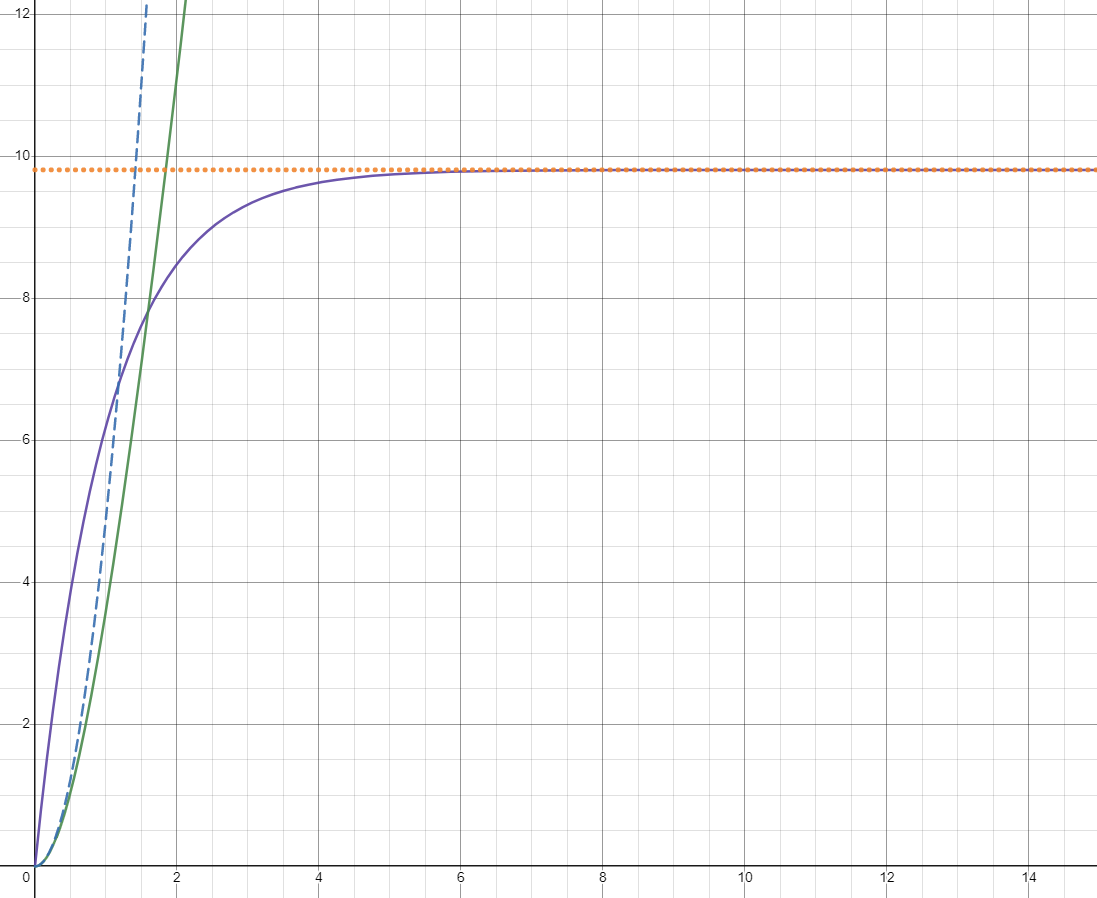
\includegraphics[height=0.8\textheight]{images/free-fall-with-air-resistance-graph.png}

		\column{0.4\textwidth}
		\begin{figure}
			
\includegraphics[width=0.5\textwidth]{images/free-fall-with-air-resistance-graph-qr-code.png}
			\tiny
			\caption{\href{https://www.desmos.com/calculator/q4jcalrbob}{desmos.com/calculator/q4jcalrbob}}
		\end{figure}
	\end{columns}
\end{frame}

\begin{frame}
	\frametitle{Why should you care?}
	"Since Newton, mankind has come to realise that the
	laws of physics are always expressed in the language of
	differential equations." - Steven Strogatz
	\begin{itemize}
		\item N-body problem, Newtons's law of cooling, heat equation, wave equation\dots
		\item Radioactive decay, reaction speed\dots
		\item Population dynamics, disease spread models, wound healing\dots
	\end{itemize}
\end{frame}

\begin{frame}
	\frametitle{Pendulums}
	\begin{columns}[T]
		\column{0.75\textwidth}
		\begin{itemize}
			\item $\theta = \theta_0\cos\left(\sqrt{\frac{g}{l}}t\right)$ for small starting angles $\theta_0$
			\item Angular acceleration for any starting angle: $\frac{d^2\theta}{dt^2} = -\frac{g}{l}\sin(\theta)$
			\item That's a second order differential equation
			\item Solving it for $\theta$ is very difficult and gets us to elliptic integrals \animategraphics[autoplay,loop,height=\baselineskip]{30}{images/kujiua-gif/frame_}{00}{95}
			\item We can instead solve it numerically
		\end{itemize}

		\column{0.25\textwidth}
		\centering
		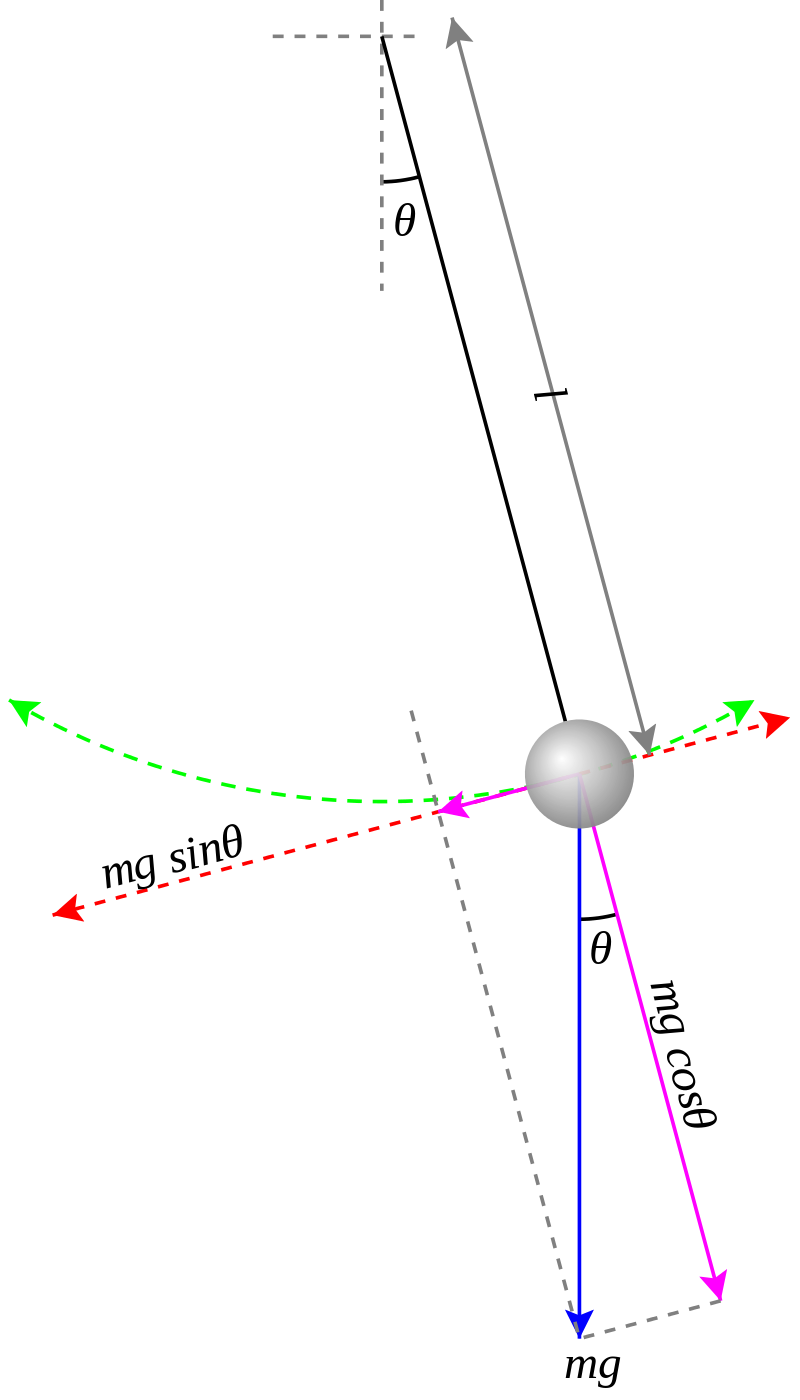
\includegraphics[height=0.75\textheight]{images/pendulum-diagram.png}
	\end{columns}
\end{frame}

\begin{frame}[fragile]
	\frametitle{Solving differential equations numerically}
	\begin{itemize}
		\item Take small steps in time and evaluate the equation
	\end{itemize}

	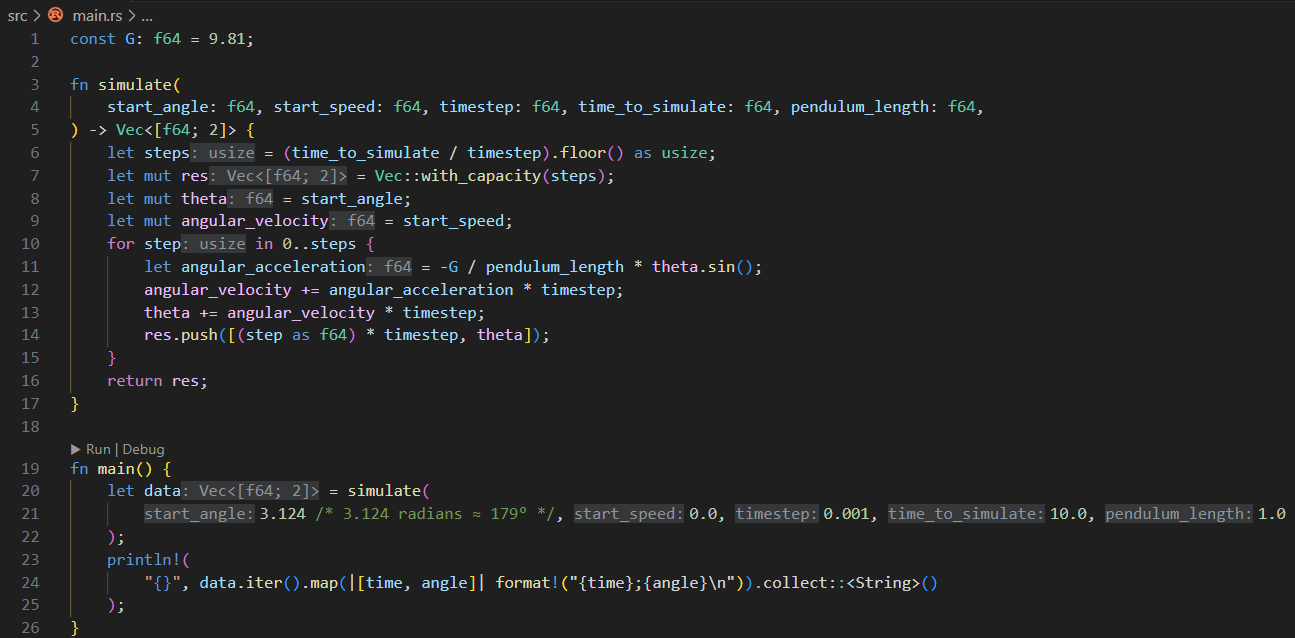
\includegraphics[width=0.78\textwidth]{images/pendulum-raw-calculation-code.png}
\end{frame}

\begin{frame}
	\frametitle{The results}
	\begin{columns}[T]
		\column{0.5\textwidth}
		\centering
		\only<1>{
			\begin{figure}
				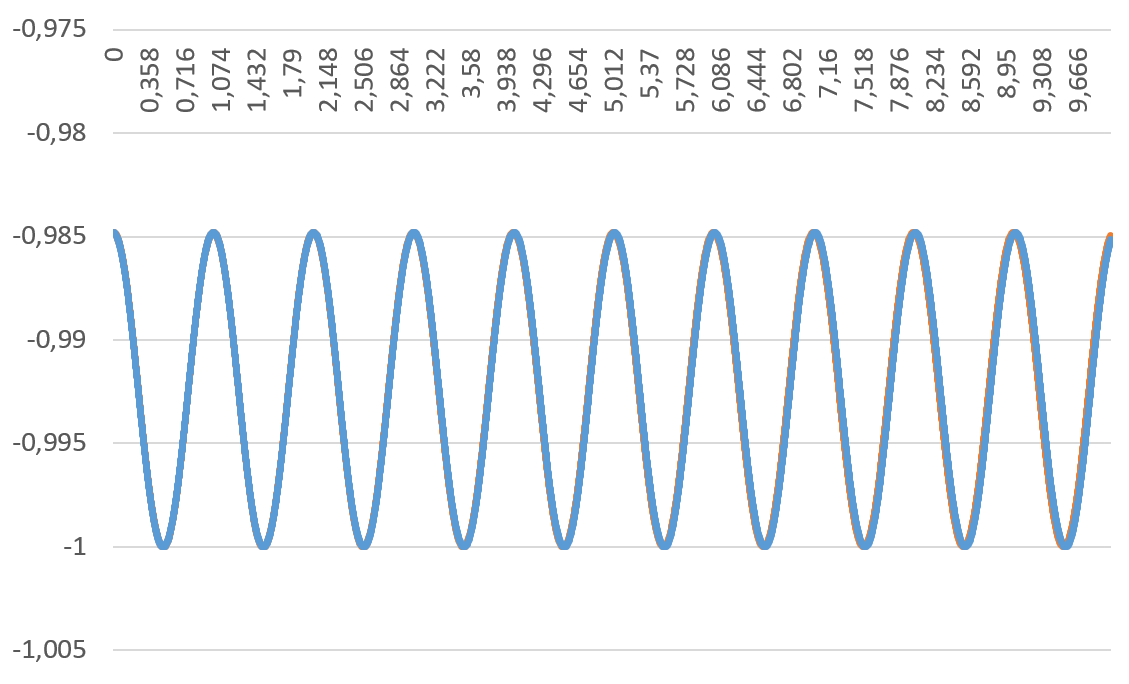
\includegraphics[width=\textwidth]{images/pendulum-calculation-graphs/displacement-10-deg.png}
				\caption{Displacement, $\theta_0 = 10^{\circ}$}
			\end{figure}
		}
		\only<2>{
			\begin{figure}
				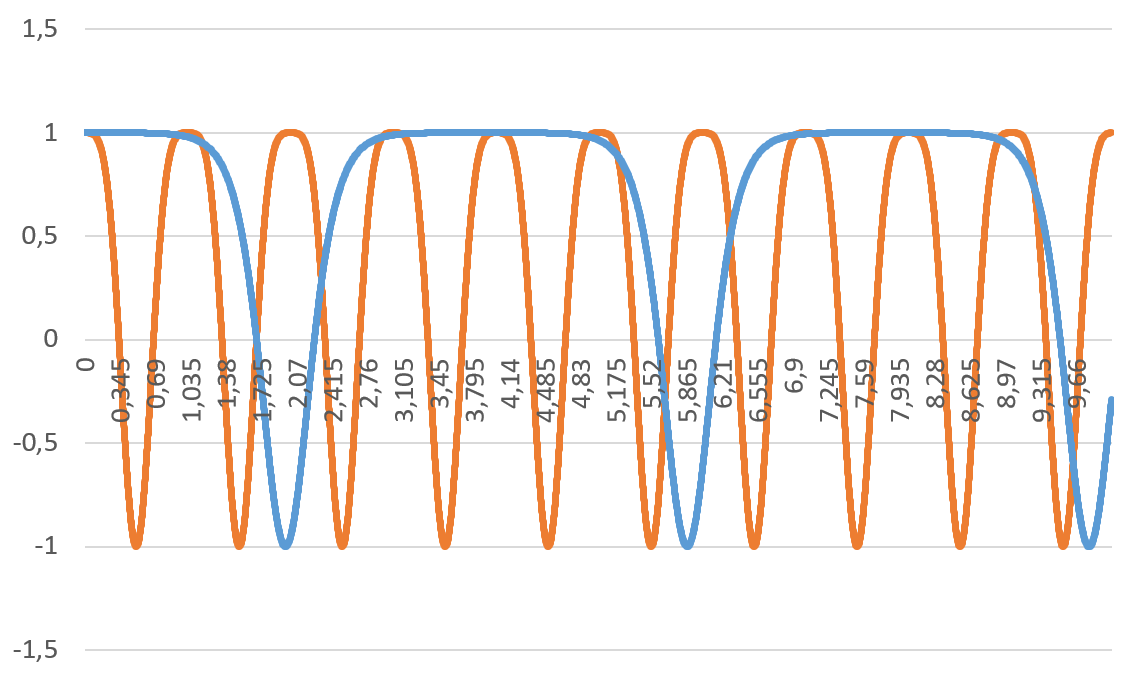
\includegraphics[width=\textwidth]{images/pendulum-calculation-graphs/displacement-179-deg.png}
				\caption{Displacement, $\theta_0 = 179^{\circ}$}
			\end{figure}
		}

		\column{0.5\textwidth}
		\centering
		\only<1>{
			\begin{figure}
				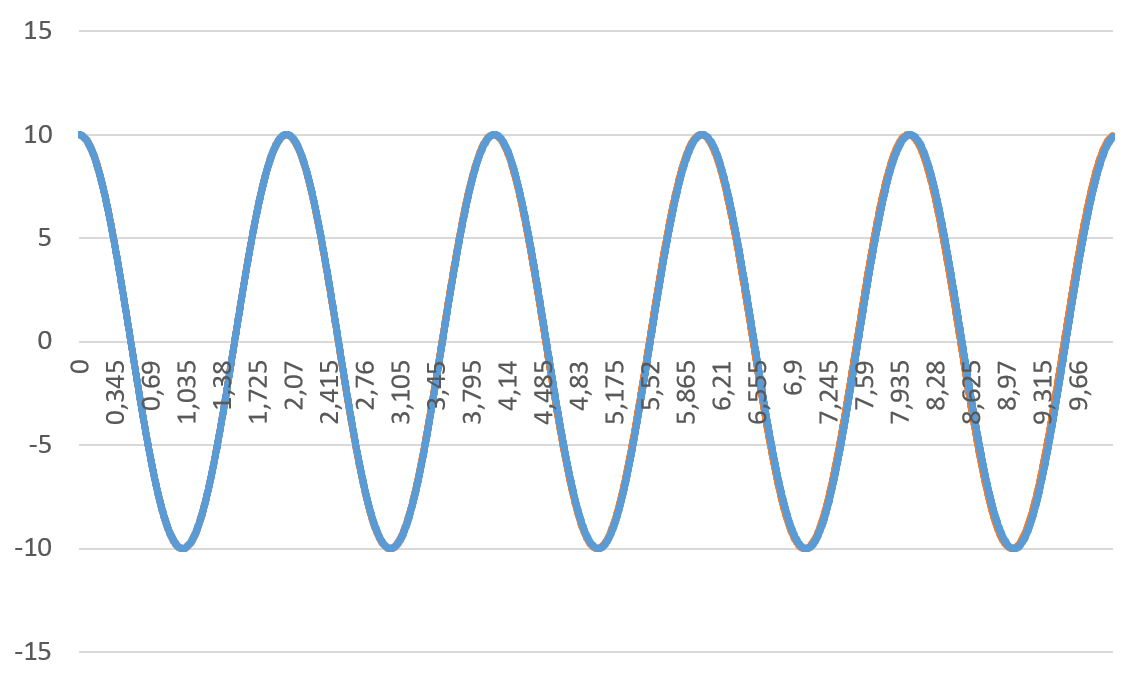
\includegraphics[width=\textwidth]{images/pendulum-calculation-graphs/angle-10-deg.png}
				\caption{Angle, $\theta_0 = 10^{\circ}$}
			\end{figure}
		}
		\only<2>{
			\begin{figure}
				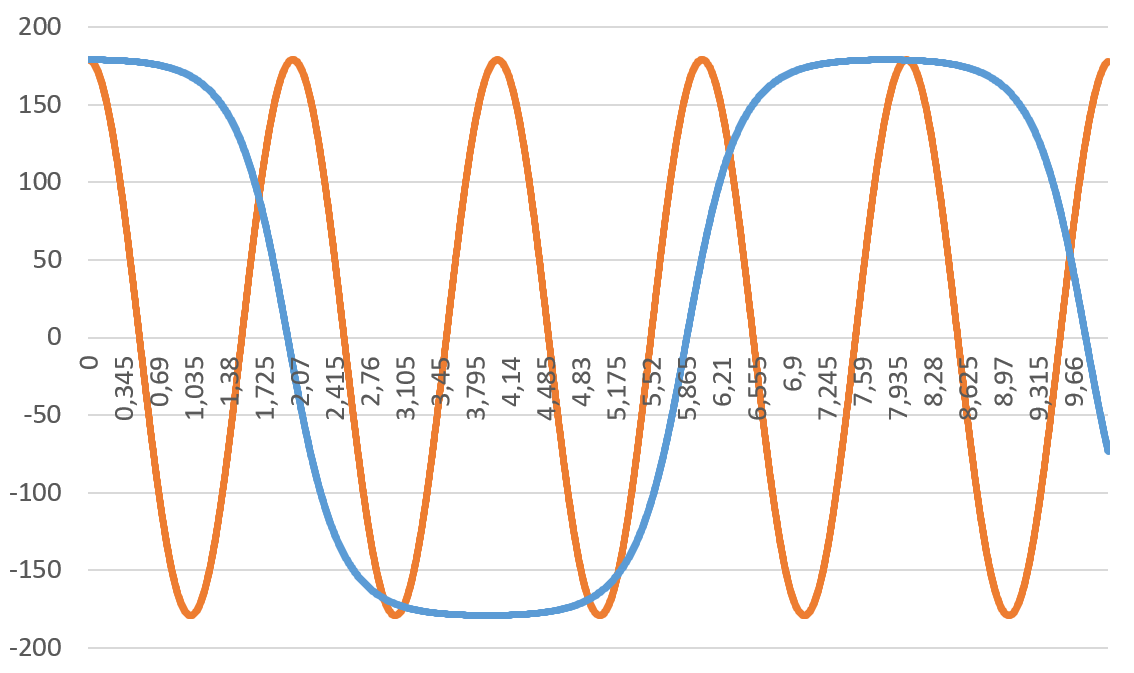
\includegraphics[width=\textwidth]{images/pendulum-calculation-graphs/angle-179-deg.png}
				\caption{Angle, $\theta_0 = 179^{\circ}$}
			\end{figure}
		}
	\end{columns}
\end{frame}

\begin{frame}
	\frametitle{Pendulum simulation}
	\centering
	\animategraphics[autoplay,loop,height=0.8\textheight]{30}{images/pendulum-simulation-gif/}{01}{56}
\end{frame}

\begin{frame}
	\frametitle{The source code, simulations, and data}
	\centering
	\begin{figure}
		
\includegraphics[height=0.6\textheight]{images/source-code-qr-code.png}
		\tiny
		\caption{\href{https://github.com/Pandicon/Pendulums-and-Differential-Equations-presentation-June-2023}{github.com/Pandicon/Pendulums-and-Differential-Equations-presentation-June-2023}}
	\end{figure}
\end{frame}

\end{document}